%%%%(c)
%%%%(c)  This file is a portion of the source for the textbook
%%%%(c)
%%%%(c)    Abstract Algebra: Theory and Applications
%%%%(c)    Copyright 1997 by Thomas W. Judson
%%%%(c)
%%%%(c)  See the file COPYING.txt for copying conditions
%%%%(c)
%%%%(c)
\chap{Finite Fields}{finite}


Finite fields appear in many applications of algebra, including coding theory and cryptography.  We already know one finite field, ${\mathbb Z}_p$, where $p$ is prime.  In this chapter we will show that a unique finite field of order $p^n$ exists for every prime $p$, where $n$ is a positive integer.  Finite fields are also called Galois fields in honor of \'{E}variste Galois, who was one of the first mathematicians to
investigate them.

 
\section{Structure of a Finite Field}

Recall that a field $F$ has {\bfi characteristic} $p$ if $p$ is the smallest positive integer such that for every nonzero element $\alpha$ in $F$, we have $p \alpha = 0$.  If no such integer exists, then $F$ has characteristic 0.  From Theorem~\ref{rings:characteristic_theorem} we know that $p$ must be prime.  Suppose that $F$ is a finite field with $n$ elements. Then $n \alpha = 0$ for all $\alpha$ in $F$.  Consequently, the characteristic of $F$ must be $p$, where $p$ is a prime dividing $n$.  This discussion is summarized in the following proposition.   

\begin{proposition}
If $F$ is a finite field, then the characteristic of $F$ is $p$, where $p$ is prime.
\end{proposition}

Throughout this chapter we will assume that $p$ is a prime number unless otherwise stated.  

\begin{proposition}
If $F$ is a finite field of characteristic $p$, then the order of $F$ is $p^n$ for some $n \in {\mathbb N}$.   
\end{proposition}

\begin{proof}
Let $\phi : {\mathbb Z} \rightarrow F$ be the ring homomorphism defined by $\phi(n) = n \cdot 1$.  Since the characteristic of $F$ is $p$, the kernel of $\phi$ must be $p {\mathbb Z}$ and the image of $\phi$ must be a subfield of $F$ isomorphic to ${\mathbb Z}_p$.  We will denote this subfield by $K$.  Since $F$ is a finite field, it must be a finite extension of $K$ and, therefore, an algebraic extension of $K$. Suppose that $[F : K] = n$ is the dimension of $F$, where $F$ is a $K$ vector space.  There must exist elements $\alpha_1, \ldots, \alpha_n \in F$ such that any element $\alpha$ in $F$ can be written uniquely in the form   
\[
\alpha = a_1 \alpha_1 + \cdots + a_n \alpha_n,
\]
where the $a_i$'s are in $K$.  Since there are $p$ elements in $K$, there are $p^n$ possible linear combinations of the $\alpha_i$'s.  Therefore, the order of $F$ must be $p^n$.  
\end{proof}

\begin{lemma}[Freshman's Dream]\index{Freshman's Dream}\label{finite:freshmans_dream}
Let $p$ be prime and $D$ be an integral domain of characteristic $p$.  Then
\[
a^{p^n} + b^{p^n} = (a + b)^{p^n}
\]
for all positive integers $n$.  
\end{lemma}

\begin{proof}
We will prove this lemma using mathematical induction on $n$.  We can use the binomial formula (see Chapter~\ref{integers}, Example~\ref{example:integers:binomial_theorem}) to verify the case for $n = 1$; that is,
\[
(a+b)^p 
= 
\sum_{k=0}^{p} 
\binom{p}{k}
a^k b^{p-k}.
\]
If $0 < k < p$, then
\[
\binom{p}{k}
=
\frac{p!}{k!(p-k)!}
\]
must be divisible by $p$, since $p$ cannot divide $k!(p - k)!$.  Note that $D$ is an integral domain of characteristic $p$, so all but the first and last terms in the sum must be zero.  Therefore, $(a + b)^p =
a^p + b^p$.  

Now suppose that the result holds for all $k$, where $1 \leq k \leq n$.  By the induction hypothesis,
\[
(a + b)^{p^{n + 1}}
=
((a + b)^p)^{p^{n}}
=
(a^p + b^p)^{p^{n}}
=
(a^p)^{p^{n}} + (b^p)^{p^{n}}
=
a^{p^{n + 1}} + b^{p^{n + 1}}.
\]
Therefore, the lemma is true for $n + 1$ and the proof is complete.
\end{proof}

\medskip

Let $F$ be a field.  A polynomial $f(x) \in F[x]$ of degree $n$ is {\bfi separable\/}\index{Polynomial separable} if it has $n$ distinct roots in the splitting field of $f(x)$; that is, $f(x)$ is separable when it factors into distinct linear factors over the splitting field of $f$.  An extension $E$ of $F$ is a {\bfi separable extension\/}\index{Extension!separable} of $F$ if every element in $E$ is the root of a separable polynomial in $F[x]$.   

%Corrected typo.  Suggested by C. Wall. - TWJ 5/15/2012

\begin{example}{}
The polynomial $x^2 - 2$ is separable over ${\mathbb Q}$ since it factors as $(x - \sqrt{2}\, )(x + \sqrt{2}\, )$. In fact, ${\mathbb Q}(\sqrt{2}\, )$ is a separable extension of ${\mathbb Q}$.  Let $\alpha =  a + b \sqrt{2}$ be any element in ${\mathbb Q}(\sqrt{2}\, )$. If $b = 0$, then $\alpha$ is a root of $x - a$.  If $b \neq 0$, then $\alpha$ is the root  of the separable polynomial 
\[
x^2 - 2 a x + a^2 - 2 b^2 = (x - (a + b \sqrt{2}\, ))(x - (a - b \sqrt{2}\, )).
\]
\end{example}
%Notation error corrected.  Suggested by C. Wall.  TWJ 5/15/2012
 
Fortunately, we have an easy test to  determine the separability of any polynomial.  Let
\[
f(x) = a_0 + a_1 x + \cdots + a_n x^n
\]
be any polynomial in  $F[x]$. Define the {\bfi derivative\/}\index{Derivative} of $f(x)$ to be 
\[
f'(x) = a_1  + 2 a_2 x + \cdots + n a_n x^{n-1}.
\]

\begin{lemma}\label{finite:separable_derivative_lemma}
Let $F$ be a field and $f(x) \in F[x]$.  Then $f(x)$ is separable if and only if $f(x)$ and $f'(x)$ are relatively prime. 
\end{lemma}


\begin{proof}
Let $f(x)$ be separable.  Then $f(x)$ factors over some extension field of $F$ as $f(x) = (x - \alpha_1) (x - \alpha_2) \cdots (x - \alpha_n)$, where $\alpha_i \neq \alpha_j$ for $i \neq j$. Taking the derivative
of $f(x)$, we see that
\begin{align*}
f'(x) & =  (x - \alpha_2) \cdots (x - \alpha_n) \\
&  +  (x - \alpha_1) (x - \alpha_3) \cdots (x - \alpha_n) \\
&  + \cdots + (x - \alpha_1) \cdots (x - \alpha_{n - 1}).
\end{align*}
Hence, $f(x)$ and $f'(x)$ can have no common factors.

To prove the converse, we will show that the contrapositive of the statement is true.  Suppose that $f(x) = (x - \alpha)^k g(x)$, where $k > 1$.  Differentiating, we have
\[
f'(x) = k ( x - \alpha)^{k-1} g(x) + (x- \alpha)^k g'(x).
\]
Therefore, $f(x)$ and $f'(x)$ have a common factor.
\end{proof}


\begin{theorem}\label{finite:splitting_field_theorem}
For every  prime $p$ and every positive integer $n$, there exists a finite field $F$ with $p^n$ elements. Furthermore, any field of order $p^n$ is isomorphic to the splitting field of $x^{p^n} -x$ over ${\mathbb Z}_p$.
\end{theorem}
 
%% TWJ 11/20/2011
%% Reference to Lemma 22.4 corrected in proof.  Suggested by A. Johnston.

\begin{proof}
Let $f(x) = x^{p^n} - x$ and let $F$ be the splitting field of $f(x)$.  Then by Lemma~\ref{finite:separable_derivative_lemma}, $f(x)$ has $p^n$ distinct zeros in $F$, since $f'(x) = p^n x^{p^n - 1} - 1 = -1$ is relatively prime to $f(x)$.  We claim that the roots of $f(x)$ form a subfield of $F$.  Certainly 0 and 1 are zeros of $f(x)$.  If $\alpha$ and $\beta$ are zeros of $f(x)$, then $\alpha + \beta$ and $\alpha \beta$ are also zeros of $f(x)$, since $\alpha^{p^n} + \beta^{p^n} =  (\alpha + \beta)^{p^n}$ and $\alpha^{p^n} \beta^{p^n} = (\alpha \beta)^{p^n}$. We also need to show that the additive inverse and the multiplicative inverse of each root of $f(x)$ are roots of $f(x)$.  For any zero $\alpha$ of $f(x)$, $-\alpha = (p - 1)\alpha$ is also a zero of $f(x)$. If $\alpha \neq 0$, then $(\alpha^{-1})^{p^n} = (\alpha^{p^n})^{-1} = \alpha^{-1}$. Since the zeros of $f(x)$ form a subfield of $F$ and $f(x)$ splits in this subfield, the subfield must be all of $F$. 

Let $E$ be any other field of order $p^n$.  To show that $E$ is isomorphic to $F$, we must show that every element in $E$ is a root of $f(x)$.  Certainly 0 is a root of $f(x)$.  Let $\alpha$ be a nonzero element of $E$.  The order of the multiplicative group of nonzero elements of $E$ is $p^n-1$; hence, $\alpha^{p^n-1} =1$ or $\alpha^{p^n} -\alpha = 0$.  Since $E$ contains $p^n$ elements, $E$ must be a splitting field of $f(x)$; however, by Corollary~\ref{fields:splitting_field_corollary}, the splitting field of any polynomial is unique up to isomorphism. 
\end{proof}
 
\medskip

The unique finite field with $p^n$ elements is called the {\bfi Galois field\/}\index{Galois field}\index{Field!Galois} of order $p^n$. We will denote this field by $\gf(p^n)$\label{galoisfield}. 

\begin{theorem}\label{finite:subfields_theorem}
Every subfield of the Galois field $\gf(p^n)$ has $p^m$ elements, where $m$ divides $n$.  Conversely, if $m \mid n$ for $m > 0$, then  there exists a unique subfield of $\gf(p^n)$ isomorphic to  $\gf(p^m)$.
\end{theorem}

\begin{proof}
Let $F$ be a subfield of $E = \gf(p^n)$.  Then $F$ must be a field extension of $K$ that contains  $p^m$ elements, where $K$ is isomorphic to ${\mathbb Z}_p$.   Then $m \mid n$, since $[E:K] = [E:F][F:K]$.

To prove the converse, suppose that $m \mid n$ for some $m > 0$.  Then $p^m -1$ divides $p^n -1$. Consequently, $x^{p^m -1} - 1$ divides $x^{p^n -1} -1$. Therefore, $x^{p^m} - x$ must divide $x^{p^n} - x$, and every zero of $x^{p^m} - x$ is also a zero of $x^{p^n} - x$. Thus, $\gf(p^n)$ contains, as a subfield, a splitting field of $x^{p^m} - x$, which must be isomorphic to $\gf(p^m)$.
\end{proof}
     

% 2010/05/18 R Beezer, added space before Figure citation
\begin{example}{GF_p24}
The lattice of subfields of $\gf(p^{24})$ is given in Figure~\ref{FieldLattice}.

\begin{figure}
\begin{center}
\tikzpreface{finite_subfield_lattice}
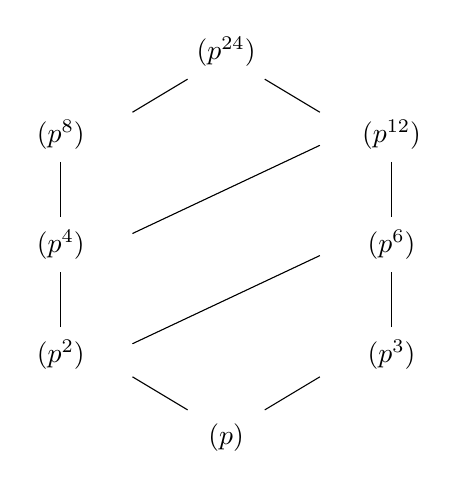
\begin{tikzpicture}[scale=0.7] %Replaced figure with tikz figure - TWJ 8/20/2010


\draw  (1.7,2.4) -- (0.7,3);
\draw  (-1.7,2.4) -- (-0.7,3);
\draw  (1.7,-2.4) -- (0.7,-3);
\draw  (-1.7,-2.4) -- (-0.7,-3);

\draw (3,1.5) -- (3,0.5);
\draw (-3,1.5) -- (-3,0.5);
\draw (3,-1.5) -- (3,-0.5);
\draw (-3,-1.5) -- (-3,-0.5);

\draw (-1.7,0.2) -- (1.7,1.8);
\draw (-1.7,-1.8) -- (1.7,-0.2);

\node at (0, 3.5) {$\gf(p^{24})$};

\node at (3, 2) {$\gf(p^{12})$};
\node at (3, 0) {$\gf(p^{6})$};
\node at (3, -2) {$\gf(p^{3})$};

\node at (-3, 2) {$\gf(p^{8})$};
\node at (-3, 0) {$\gf(p^{4})$};
\node at (-3, -2) {$\gf(p^{2})$};

\node at (0, -3.5) {$\gf(p)$};

\end{tikzpicture}
\end{center}
\caption{Subfields of $\gf(p^{24})$}
\label{FieldLattice}
\end{figure}

\end{example}
 


With each field $F$ we have a multiplicative group of nonzero elements of $F$ which we will denote by $F^*$\label{ntmultgrp}.   The multiplicative group of any finite field is cyclic.  This result follows from the more general result that we will prove in the next theorem. 

\begin{theorem}\label{finite:mult_group_theorem}
If $G$ is a finite  subgroup of $F^\ast$, the multiplicative group of nonzero elements of a field $F$, then $G$ is cyclic. 
\end{theorem}
 

\begin{proof}
Let $G$ be a finite subgroup of $F^\ast$ of order $n$.  By the Fundamental Theorem of Finite Abelian Groups (Theorem \ref{struct:Finite_Abelian_Grps_Theorem}),  
\[
G \cong {\mathbb Z}_{p_1^{e_1}} \times \cdots \times {\mathbb Z}_{p_k^{e_k}},
\]
where $n = p_1^{e_1} \cdots p_k^{e_k}$ and the  $p_1, \ldots, p_k$ are (not necessarily distinct) primes.
Let $m$ be the least common multiple of $p_1^{e_1}, \ldots, p_k^{e_k}$.  Then $G$ contains an element of order $m$.  Since every $\alpha$ in $G$ satisfies $x^r - 1$ for some $r$ dividing $m$, $\alpha$ must also be a root of $x^m - 1$.  Since $x^m -1$ has at most $m$ roots in $F$, $n \leq m$.  On the other hand, we know that $m \leq |G|$; therefore, $m = n$. Thus, $G$ contains an element of order $n$ and must be cyclic. 
\end{proof}

%Rewrote the first part of the proof.  Suggested by R. Beezer.
%TWK - 24/4/2013

\begin{corollary}\label{finite:cyclic_corollary}
The multiplicative group of all nonzero elements of a finite field is cyclic. 
\end{corollary}

\begin{corollary}\label{finite:finite_extension_corollary}
Every finite extension $E$ of a finite field $F$ is a simple extension of $F$. 
\end{corollary}

\begin{proof}
Let $\alpha$ be a generator for the cyclic group $E^{\ast}$ of nonzero elements of $E$. Then $E = F( \alpha )$. 
\end{proof}
 

\begin{example}{GF_2^4}
The finite field $\gf(2^4)$ is isomorphic to the field ${\mathbb Z}_2/ \langle 1 + x + x^4 \rangle$. Therefore, the elements of  $\gf(2^4)$ can be taken to be
\[
\{
a_0 + a_1 \alpha + a_2 \alpha^2 + a_3 \alpha^3 : a_i \in {\mathbb Z}_2
\text{ and } 1 + \alpha + \alpha^4 = 0
\}.
\]
Remembering that $1 + \alpha +\alpha^4 = 0$, we add and multiply elements of $\gf(2^4)$ exactly as we add and multiply polynomials.  The multiplicative group of $\gf(2^4)$ is isomorphic to ${\mathbb  Z}_{15}$ with generator $\alpha$: 
\[
\begin{array}{rclcrclcrcl}
\alpha^1 & = & \alpha & &
\alpha^6  & = & \alpha^2 + \alpha^3 & &
\alpha^{11} & = & \alpha + \alpha^2 + \alpha^3 \\
\alpha^2 & = & \alpha^2 & &
\alpha^7  & = & 1 + \alpha + \alpha^3 & &
\alpha^{12} & = & 1 + \alpha + \alpha^2 + \alpha^3 \\
\alpha^3 & = & \alpha^3 & &
\alpha^8  & = & 1 + \alpha^2 & &
\alpha^{13} & = & 1 + \alpha^2 + \alpha^3 \\
\alpha^4 & = & 1 + \alpha & &
\alpha^9  & = & \alpha + \alpha^3 & &
\alpha^{14} & = & 1 + \alpha^3 \\
\alpha^5 & = & \alpha + \alpha^2 & &
\alpha^{10}  & = & 1 + \alpha + \alpha^2 & &
\alpha^{15} & = & 1. 
\end{array}
\]
\end{example}


\section{Polynomial Codes}

%TWJ 2012/11/21
%Chapter reference updated.  Suggested by J. Buller.

With knowledge of polynomial rings and finite fields, it is now possible to derive more sophisticated codes than those of Chapter~\ref{algcodes}.  First let us recall that an $(n, k)$-block code consists of a one-to-one encoding function $E:{\mathbb Z}^{k}_{2} \rightarrow {\mathbb Z}^{n}_{2}$ and a decoding function $D:{\mathbb Z}^{n}_{2} \rightarrow {\mathbb Z}^{k}_{2}$.  The code is error-correcting if $D$ is onto.  A code is a linear code if it is the null space of a matrix $H \in {\mathbb M}_{k \times n}({\mathbb Z}_2)$.  

We are interested in a class of codes known as cyclic codes\index{Code!cyclic}.  Let $\phi : {\mathbb Z}_2^k \rightarrow {\mathbb  Z}_2^n$ be a binary $(n,k)$-block code.  Then $\phi$ is a {\bfi cyclic code\/} if for every codeword $(a_1, a_2, \ldots, a_n )$, the cyclically shifted $n$-tuple $(a_n, a_1, a_2, \ldots, a_{n-1} )$ is also a codeword.  Cyclic codes are particularly easy to implement on a  computer using shift registers [2, 3].  


\begin{example}{6-3-linear_code}
Consider the $(6,3)$-linear codes generated by the two matrices
\[
G_1 
= 
\begin{pmatrix}
1 & 0 & 0 \\
0 & 1 & 0 \\
0 & 0 & 1 \\
1 & 0 & 0 \\
0 & 1 & 0 \\
0 & 0 & 1 
\end{pmatrix}
\quad
\text{and}
\quad
G_2 = 
\begin{pmatrix}
1 & 0 & 0 \\
1 & 1 & 0 \\
1 & 1 & 1 \\
1 & 1 & 1 \\
0 & 1 & 1 \\
0 & 0 & 1
\end{pmatrix}.
\]
Messages in the first code are encoded as follows:
\[
\begin{array}{rclccrcl}
(000) & \mapsto & (000000) & & & (100) & \mapsto & (100100) \\
(001) & \mapsto & (001001) & & & (101) & \mapsto & (101101) \\
(010) & \mapsto & (010010) & & & (110) & \mapsto & (110110) \\
(011) & \mapsto & (011011) & & & (111) & \mapsto & (111111).
\end{array}
\]
It is easy to see that the codewords form a cyclic code.  In the second code, 3-tuples are encoded in the following manner:
\[
\begin{array}{rclccrcl}
(000) & \mapsto & (000000) & & & (100) & \mapsto & (111100) \\
(001) & \mapsto & (001111) & & & (101) & \mapsto & (110011) \\
(010) & \mapsto & (011110) & & & (110) & \mapsto & (100010) \\
(011) & \mapsto & (010001) & & & (111) & \mapsto & (101101).
\end{array}
\]
This code cannot be cyclic, since $(101101)$ is a codeword but $(011011)$ is not a codeword.
\end{example}


\subsection*{Polynomial Codes}

We would like to find an easy method of obtaining cyclic linear codes.  To accomplish this, we can use our knowledge of finite fields and  polynomial rings over ${\mathbb Z}_2$.  Any binary $n$-tuple can be
interpreted as a polynomial in ${\mathbb Z}_2[x]$.  Stated another way, the $n$-tuple $(a_0, a_1, \ldots, a_{n-1} )$ corresponds to the polynomial
\[
f(x) = a_0 +  a_1 x +  \cdots + a_{n-1} x^{n-1},
\]
where the degree of $f(x)$ is at most $n-1$.   For example, the polynomial corresponding to the 5-tuple $(10011)$ is  
\[
1 + 0 x + 0 x^2 + 1 x^3 + 1 x^4 = 1 + x^3 + x^4.
\]
Conversely, with any polynomial $f(x) \in {\mathbb Z}_2[x]$ with $\deg f(x) < n$ we can associate a binary $n$-tuple.  The polynomial $x + x^2 + x^4$ corresponds to the 5-tuple $(01101)$.

Let us fix a nonconstant polynomial $g(x)$ in ${\mathbb Z}_2[x]$ of degree \mbox{$n - k$}.  We can define an $(n,k)$-code $C$ in the following manner.  If $(a_0, \ldots, a_{k-1})$ is a $k$-tuple to be encoded, then $f(x) = a_0 + a_1 x +  \cdots + a_{k-1} x^{k-1}$ is the corresponding polynomial
in ${\mathbb Z}_2[x]$.  To encode $f(x)$, we multiply by $g(x)$.  The codewords in $C$ are all those polynomials in ${\mathbb Z}_2[x]$ of degree less than  $n$ that are divisible by $g(x)$.  Codes obtained in this manner are called {\bfi polynomial codes}\index{Polynomial!code}\index{Code!polynomial}.  


\begin{example}{generator_63-code}
If we let $g(x)= 1 + x^3$, we can define a $(6,3)$-code $C$ as follows.  To encode a 3-tuple $( a_0, a_1, a_2 )$, we multiply the corresponding polynomial $f(x) = a_0 + a_1 x + a_2 x^2$ by $1 + x^3$.  We are defining a map $\phi : {\mathbb Z}_2^3 \rightarrow {\mathbb Z}_2^6$ by $\phi  : f(x) \mapsto g(x) f(x)$.  It is easy to check that this map is a group homomorphism.  In fact, if we regard ${\mathbb Z}_2^n$ as a vector space over ${\mathbb Z}_2$, $\phi$ is a linear transformation of vector spaces (see Exercise~\ref{vect:linear_transformation}, Chapter~\ref{vect}).  Let us compute the kernel of $\phi$.  Observe that $\phi ( a_0, a_1, a_2 ) = (000000)$ exactly when 
\begin{align*}
0 + 0x + 0x^2 + 0x^3 + 0x^4 + 0 x^5 
& = (1 + x^3) ( a_0 + a_1 x + a_2 x^2 ) \\ 
& = a_0 + a_1 x + a_2 x^2 + a_0 x^3 + a_1 x^4 + a_2 x^5.
\end{align*}
Since the polynomials over a field form an integral domain, $a_0 + a_1 x + a_2 x^2$ must be the zero polynomial. Therefore, $\ker \phi = \{ (000) \}$ and $\phi$ is one-to-one. 
 

To calculate a generator matrix for $C$, we merely need to examine the way the polynomials $1$, $x$, and $x^2$ are encoded:
\begin{align*}
(1 + x^3) \cdot 1 & = 1 + x^3 \\
(1 + x^3)x & = x + x^4 \\
(1 + x^3)x^2 & = x^2 + x^5. 
\end{align*}  %Changed minimal polynomial from  (1 + x^3)x^3 & = x^2 + x^5 to (1 + x^3)x^2 & = x^2 + x^5.  Discovered by Jon Buller - TWJ 3/25/2011
We obtain the code corresponding to the generator matrix $G_1$ in Example~\ref{example:finite:6-3-linear_code}.  The parity-check matrix for this code is
\[
H
= 
\begin{pmatrix}
1 & 0 & 0 & 1 & 0 & 0 \\
0 & 1 & 0 & 0 & 1 & 0 \\
0 & 0 & 1 & 0 & 0 & 1 
\end{pmatrix}.
\]
Since the smallest weight of any nonzero codeword is 2, this code has the ability to detect all single errors.  
\end{example}


Rings of polynomials have a great deal of structure; therefore, our immediate goal is to establish a link between polynomial codes and ring theory. Recall that $x^n - 1 = (x - 1)( x^{n-1} + \cdots + x + 1)$.  The factor ring 
\[
R_n = {\mathbb Z}_2[x]/ \langle x^n - 1 \rangle
\] 
can be considered to be the ring of polynomials of the form 
\[
f(t) = a_0 + a_1 t + \cdots + a_{n-1} t^{n-1}
\]
that satisfy the condition $t^n = 1$.  It is an easy exercise to show that ${\mathbb Z}_2^n$ and $R_n$ are isomorphic as vector spaces.  We will often identify elements in ${\mathbb Z}_2^n$ with elements in
${\mathbb Z}[x] / \langle x^n - 1 \rangle$.  In this manner we can interpret a linear code as a subset of ${\mathbb Z}[x] / \langle x^n - 1 \rangle$.  

The additional ring structure on polynomial codes is very powerful in describing cyclic codes. A cyclic shift of an $n$-tuple can be described by polynomial multiplication.  If $f(t) = a_0 + a_1 t + \cdots + a_{n-1} t^{n-1}$ is a code polynomial in $R_n$, then
\[
tf(t) = a_{n-1} + a_0 t + \cdots + a_{n-2} t^{n-1}
\]
is the cyclically shifted word obtained from multiplying $f(t)$ by $t$.  The following theorem gives a beautiful classification of cyclic codes in terms of the ideals of $R_n$.

\begin{theorem} \label{finite:cyclic_code_theorem}
A linear code $C$ in ${\mathbb Z}_2^n$ is cyclic if and only if it is an ideal in $R_n = {\mathbb Z}[x] / \langle x^n - 1 \rangle$. 
\end{theorem}
 
\begin{proof}
Let $C$ be a linear cyclic code and suppose that $f(t)$ is in $C$.  Then $t f(t)$ must also be in $C$. Consequently, $t^k f(t)$ is in $C$ for all $k \in {\mathbb N}$.  Since $C$ is a linear code, any linear combination of the codewords $f(t), tf(t), t^2f(t), \ldots, t^{n-1}f(t)$ is also a codeword; therefore, for every polynomial $p(t)$, $p(t)f(t)$ is in $C$.  Hence, $C$ is an ideal. 

Conversely, let $C$ be an ideal in ${\mathbb Z}_2[x]/\langle x^n + 1\rangle$. Suppose that $f(t) = a_0 + a_1 t + \cdots + a_{n - 1} t^{n - 1}$ is a codeword in $C$.  Then $t f(t)$ is a codeword in $C$; that is, $(a_1, \ldots, a_{n-1}, a_0)$ is in $C$.
\end{proof} 

\medskip

Theorem~\ref{finite:cyclic_code_theorem} tells us that knowing the ideals of $R_n$ is equivalent to knowing the linear cyclic codes in ${\mathbb Z}_2^n$.  Fortunately, the ideals in $R_n$ are easy to describe.  The  natural ring homomorphism $\phi : {\mathbb Z}_2[x] \rightarrow R_n$ defined by $\phi[f(x)] = f(t)$ is a surjective homomorphism.  The kernel of $\phi$ is the ideal generated by $x^n - 1$.  By Theorem~\ref{rings:correspond_theorem}, every ideal $C$ in $R_n$ is of the form $\phi(I)$, where $I$ is an ideal in ${\mathbb Z}_2[x]$ that contains $\langle x^n - 1 \rangle$.  By Theorem~\ref{poly:PI_theorem}, we know that every ideal $I$ in ${\mathbb Z}_2[x]$ is a principal ideal, since ${\mathbb Z}_2$ is a field. Therefore, $I = \langle g(x) \rangle$ for some unique monic polynomial in ${\mathbb Z}_2[x]$. Since $\langle x^n - 1 \rangle$ is contained in $I$, it must be the case that $g(x)$ divides $x^n - 1$. Consequently, every ideal $C$ in $R_n$ is of the form 
\[
C= \langle g(t) \rangle = \{ f(t)g(t) : f(t) \in R_n \mbox{ and $g(x)
\mid (x^n - 1)$ in } {\mathbb Z}_2[x] \}.
\] 
The unique monic polynomial of the smallest degree that generates $C$ is called the {\bfi minimal generator polynomial\/}\index{Minimal generator polynomial}\index{Polynomial!minimal generator} of $C$. 


\begin{example}{factor_x7-1}
If we factor $x^7 - 1$ into irreducible components, we have
\[
x^7 - 1 = (1 + x)(1 + x + x^3)(1+ x^2 + x^3).
\]
We see that $g(t) = (1 + t + t^3)$ generates an ideal $C$ in $R_7$.  This code is a $(7, 4)$-block code.  As in Example~\ref{example:finite:generator_63-code}, it is easy to calculate a generator matrix by examining what $g(t)$ does to the polynomials 1, $t$, $t^2$, and $t^3$.  A generator matrix for $C$ is 
\[
G =
\begin{pmatrix}
1 & 0 & 0 & 0 \\
1 & 1 & 0 & 0 \\
0 & 1 & 1 & 0 \\
1 & 0 & 1 & 1 \\
0 & 1 & 0 & 1 \\
0 & 0 & 1 & 0 \\
0 & 0 & 0 & 1
\end{pmatrix}.
\]
\end{example}

 
In general, we can determine a generator matrix for an $(n, k)$-code $C$ by the manner in which the elements $t^k$ are encoded. Let $x^n - 1 = g(x) h(x)$ in ${\mathbb Z}_2[x]$. If $g(x) = g_0 + g_1 x + \cdots + g_{n-k} x^{n-k}$ and $h(x) = h_0 + h_1 x +  \cdots + h_k x^k$, then the $n \times k$ matrix
\[
G = 
\begin{pmatrix}
g_0 & 0   & \cdots & 0 \\
g_1 & g_0 & \cdots & 0 \\
\vdots & \vdots &\ddots & \vdots \\
g_{n-k}   & g_{n-k-1} & \cdots & g_0 \\
0   & g_{n-k} & \cdots & g_{1} \\
\vdots & \vdots & \ddots & \vdots \\
0   & 0 & \cdots & g_{n-k}
\end{pmatrix}
\]
is a generator matrix for the code $C$ with generator polynomial $g(t)$.  The parity-check matrix for $C$ is the $(n-k) \times n$ matrix 
\[
H =
\begin{pmatrix}
0   & \cdots & 0   & 0      & h_k    & \cdots & h_0 \\
0   & \cdots & 0 & h_k & \cdots & h_0    & 0 \\
\cdots  & \cdots & \cdots  & \cdots &  \cdots &  \cdots & \cdots \\
h_k & \cdots & h_0 & 0      & 0      & \cdots & 0 
\end{pmatrix}.
\]
We will leave the details of the proof of the following proposition as an exercise.  

\begin{proposition}
Let $C = \langle g(t) \rangle$ be a cyclic code in $R_n$ and suppose that $x^n - 1 = g(x) h(x)$.  Then $G$ and $H$ are generator and parity-check matrices  for $C$, respectively.  Furthermore, $HG = 0$. 
\end{proposition}


\begin{example}{parity-check}
In Example~\ref{example:finite:factor_x7-1},
\[
x^7 - 1 = g(x) h(x) = (1 + x + x^3)(1 + x + x^2 + x^4).
\]
Therefore, a parity-check matrix for this code is
\[
H =
\begin{pmatrix}
0 & 0 & 1 & 0 & 1 & 1 & 1 \\
0 & 1 & 0 & 1 & 1 & 1 & 0 \\
1 & 0 & 1 & 1 & 1 & 0 & 0
\end{pmatrix}.
\]
\end{example}


To determine the error-detecting and error-correcting capabilities of a cyclic code, we need to know something about determinants.  If $\alpha_1, \ldots, \alpha_n$ are elements in a field $F$, then the $n 
\times n$ matrix  
\[
\begin{pmatrix}
1          & 1          & \cdots & 1 \\
\alpha_1   & \alpha_2   & \cdots & \alpha_n \\
\alpha_1^2 & \alpha_2^2 & \cdots & \alpha_n^2 \\
\vdots     & \vdots     & \ddots & \vdots \\
\alpha_1^{n-1} & \alpha_2^{n-1} & \cdots & \alpha_n^{n-1} 
\end{pmatrix}
\]
is called the {\bfi Vandermonde matrix}\index{Vandermonde matrix}\index{Matrix, Vandermonde}.  The
determinant of this matrix is called the {\bfi Vandermonde determinant}\index{Vandermonde determinant}\index{Determinant, Vandermonde}.  We will need the following lemma in our investigation of cyclic codes.

\begin{lemma}\label{finite:V_det_lemma}
Let $\alpha_1, \ldots, \alpha_n$ be elements in a field $F$ with $n \geq 2$.  Then
\[
\det
\begin{pmatrix}
1              & 1              & \cdots & 1 \\
\alpha_1       & \alpha_2       & \cdots & \alpha_n \\
\alpha_1^2     & \alpha_2^2     & \cdots & \alpha_n^2 \\
\vdots         & \vdots         & \ddots & \vdots \\
\alpha_1^{n-1} & \alpha_2^{n-1} & \cdots & \alpha_n^{n-1} 
\end{pmatrix}
= 
\prod_{1 \leq j < i \leq n} (\alpha_i - \alpha_j).
\]
In particular, if the $\alpha_i$'s are distinct, then the determinant is nonzero.
\end{lemma}


\begin{proof}
We will induct on $n$. If $n = 2$, then the determinant is $\alpha_2 - \alpha_1$.  Let us assume the result for $n  - 1$ and consider the polynomial $p(x)$ defined~by
\[
p(x)
=
\det
\begin{pmatrix}
1              & 1              & \cdots & 1              & 1 \\
\alpha_1       & \alpha_2       & \cdots & \alpha_{n-1}   & x \\
\alpha_1^2     & \alpha_2^2     & \cdots & \alpha_{n-1}^2 & x^2 \\
\vdots         & \vdots         & \ddots & \vdots         & \vdots \\
\alpha_1^{n-1} & \alpha_2^{n-1} & \cdots & \alpha_{n-1}^{n-1} & x^{n-1}
\end{pmatrix}.
\]
Expanding this determinant by cofactors on the last column, we see that $p(x)$ is a polynomial of at most degree $n-1$.  Moreover, the roots of $p(x)$ are $\alpha_1, \ldots, \alpha_{n-1}$, since the substitution of any one of these elements in the last column will produce a column identical to the last column in the matrix.  Remember that the determinant of a matrix is zero if it has two identical columns. Therefore,     
\[
p(x) = (x - \alpha_1)(x - \alpha_2) \cdots (x - \alpha_{n-1}) \beta, 
\]
where
\[
\beta = (-1)^{n+n}
\det
\begin{pmatrix}
1              & 1              & \cdots & 1 \\
\alpha_1       & \alpha_2       & \cdots & \alpha_{n-1} \\
\alpha_1^2     & \alpha_2^2     & \cdots & \alpha_{n-1}^2 \\
\vdots         & \vdots         & \ddots & \vdots \\
\alpha_1^{n-2} & \alpha_2^{n-2} & \cdots & \alpha_{n-1}^{n-2} 
\end{pmatrix}.
\]
By our induction hypothesis,
\[
\beta = (-1)^{n+n} \prod_{1 \leq j < i \leq n-1} (\alpha_i - \alpha_j).
\]
If we let $x = \alpha_n$, the result now follows immediately.
\end{proof}

\medskip

The following theorem gives us an estimate on the error detection and correction capabilities for a particular generator polynomial.

\begin{theorem}\label{finite:min_dist_theorem}
Let $C = \langle g(t) \rangle$ be a cyclic code in $R_n$ and suppose that $\omega$ is a primitive $n$th root of unity over ${\mathbb Z}_2$.  If $s$ consecutive powers of $\omega$ are roots of $g(x)$, then the minimum distance of $C$ is at least $s+1$.
\end{theorem}


\begin{proof}
Suppose that 
\[
g( \omega^r) = g(\omega^{r+1}) = \cdots = g( \omega^{r+s-1}) = 0.
\]
Let $f(x)$ be some polynomial in $C$ with $s$ or fewer nonzero coefficients.  We can assume that 
\[
f(x) = a_{i_0} x^{i_0} + a_{i_1} x^{i_1} + \cdots + a_{i_{s-1}}
x^{i_{s-1}} 
\]
be some polynomial in $C$. It will suffice to show that all of the $a_i$'s must be 0.  Since 
\[
g( \omega^r) = g(\omega^{r+1}) = \cdots = g( \omega^{r+s-1}) = 0
\]
and $g(x)$ divides $f(x)$,
\[
f( \omega^r) = f(\omega^{r+1}) = \cdots = f( \omega^{r+s-1}) = 0.
\]
Equivalently, we have the following system of equations:
\begin{align*}
a_{i_0} (\omega^r)^{i_0} + a_{i_1} (\omega^r)^{i_1} + \cdots +
a_{i_{s-1}} (\omega^r)^{i_{s-1}} & = 0 \\ 
a_{i_0} (\omega^{r+1})^{i_0} + a_{i_1} (\omega^{r+1})^{i_2} + \cdots +
a_{i_{s-1}} (\omega^{r+1})^{i_{s-1}} & = 0 \\ 
& \vdots  \\
a_{i_0} (\omega^{r+s-1})^{i_0} + a_{i_1} (\omega^{r+s-1})^{i_1} +
\cdots + a_{i_{s-1}} (\omega^{r+s-1})^{i_{s-1}} & = 0.
\end{align*}
Therefore, $(a_{i_0}, a_{i_1}, \ldots, a_{i_{s-1}})$ is a solution to the homogeneous system of linear equations
\begin{align*}
(\omega^{i_0})^r x_0 + (\omega^{i_1})^r x_1 + \cdots +
(\omega^{i_{s-1}})^r x_{n-1} & = 0 \\ 
(\omega^{i_0})^{r+1} x_0 + (\omega^{i_1})^{r+1} x_1 + \cdots +
(\omega^{i_{s-1}})^{r+1} x_{n-1} & = 0 \\ 
& \vdots  \\
(\omega^{i_0})^{r+s-1} x_0 + (\omega^{i_1})^{r+s-1} x_1 + \cdots +
(\omega^{i_{s-1}})^{r+s-1} x_{n-1} & = 0.
\end{align*}
However, this system has a unique solution, since the determinant of the matrix
\[
\begin{pmatrix}
(\omega^{i_0})^r & (\omega^{i_1})^r & \cdots & (\omega^{i_{s-1}})^r \\
(\omega^{i_0})^{r+1} & (\omega^{i_1})^{r+1} & \cdots &
(\omega^{i_{s-1}})^{r+1} \\
\vdots & \vdots         & \ddots & \vdots \\
(\omega^{i_0})^{r+s-1} & (\omega^{i_1})^{r+s-1} & \cdots &
(\omega^{i_{s-1}})^{r+s-1} 
\end{pmatrix}
\]
can be shown to be nonzero using Lemma~\ref{finite:V_det_lemma} and the basic properties of determinants (Exercise).   Therefore, 
this solution must be $a_{i_0} = a_{i_1} = \cdots = a_{i_{s-1}} = 0$.  
\end{proof}


\subsection*{BCH Codes}
 
Some of the most important codes,
discovered independently by A.~Hocquenghem in 1959 and by R.~C. Bose and D.~V. Ray-Chaudhuri in 1960, are BCH codes.  The European and transatlantic  communication systems both use BCH codes.  Information words to be
encoded are of length 231, and a polynomial of degree 24 is used to
generate the code.  Since $231 + 24 = 255 = 2^8-1$, we are dealing
with a \mbox{$(255, 231)$-block} code. This BCH code will detect six
errors and has a failure rate of 1 in 16 million. One advantage of BCH
codes is that efficient error correction algorithms exist for them. 


The idea behind BCH codes is to choose a generator polynomial of
smallest degree that has the largest error detection and error
correction 
capabilities. Let $d = 2r + 1$ for some $r \geq 0$.  Suppose that
$\omega$ is a primitive $n$th root of unity over ${\mathbb Z}_2$, and
let $m_i(x)$ be the minimal polynomial over ${\mathbb Z}_2$ of
$\omega^i$. If  
\[
g(x) = \lcm[ m_1(x), m_{2}(x), \ldots, m_{2r}(x)],
\]
then the cyclic code $\langle g(t) \rangle$ in $R_n$ is called the
{\bfi BCH code of length}\index{Code!BCH} $n$ {\bfi and distance} $d$.
By Theorem~\ref{finite:min_dist_theorem}, the minimum distance of $C$ is at least $d$. 


\begin{theorem}
Let $C = \langle g(t) \rangle$ be a cyclic code in $R_n$. The
following statements are equivalent. 
\begin{enumerate}

\rm\item\it
The code $C$ is a BCH code whose minimum distance is at least $d$.


\rm\item\it
A code polynomial $f(t)$ is in $C$ if and only if $f( \omega^i) = 0$
for $1 \leq i < d$. 

\rm\item\it
The matrix 
\[
H
=
\begin{pmatrix}
1      & \omega      & \omega^2    & \cdots & \omega^{n-1}\\
1      & \omega^2    & \omega^{4}  & \cdots & \omega^{(n-1)(2)} \\
1      & \omega^3    & \omega^{6}  & \cdots & \omega^{(n-1)(3)} \\
\vdots & \vdots      & \vdots      & \ddots & \vdots \\
1      & \omega^{2r} & \omega^{4r} & \cdots & \omega^{(n-1)(2r)} 
\end{pmatrix}
\]
is a parity-check matrix for $C$.

\end{enumerate}
\end{theorem}


\begin{proof}
(1) $\Rightarrow$ (2).
If $f(t)$ is in $C$, then $g(x) \mid f(x)$ in ${\mathbb Z}_2[x]$. Hence,
for $i = 1, \ldots, 2r$, $f( \omega^i) = 0$ since $g( \omega^i ) =
0$. Conversely, suppose that $f( \omega^i) = 0$ for $1 \leq i \leq d$.
Then $f(x)$ is divisible by each $m_i(x)$, since $m_i(x)$ is the
minimal polynomial of $\omega^i$. Therefore, $g(x) \mid f(x)$ by the
definition of $g(x)$. Consequently, $f(x)$ is a codeword.


(2) $\Rightarrow$ (3).
Let \mbox{$f(t) = a_0 + a_1 t + \cdots + a_{n-1}v t^{n-1}$} be in $R_n$. The
corresponding $n$-tuple in ${\mathbb Z}_2^n$ is ${\mathbf x} = (a_0 a_1
\cdots a_{n-1})^{\rm t}$. By (2),
\[
H {\mathbf x}
=
\begin{pmatrix}
a_0 + a_1 \omega + \cdots + a_{n-1} \omega^{n-1} \\
a_0 + a_1 \omega^2 + \cdots + a_{n-1} (\omega^2)^{n-1} \\
\vdots \\
a_0 + a_1 \omega^{2r} + \cdots + a_{n-1} (\omega^{2r})^{n-1}
\end{pmatrix}
=
\begin{pmatrix}
f(\omega) \\
f(\omega^2) \\
\vdots \\
f(\omega^{2r})
\end{pmatrix}
=0
\]
exactly when $f(t)$ is in $C$. Thus, $H$ is a parity-check matrix for
$C$.

(3) $\Rightarrow$ (1).
By (3), a code polynomial $f(t) = a_0 + a_1 t + \cdots + a_{n-1}
t^{n-1}$ is in $C$ exactly when $f(\omega^i) = 0$ for $i = 1, \ldots,
2r$. The smallest such polynomial is $g(t) = \lcm[ m_1(t),\ldots,
m_{2r}(t)]$.  Therefore, $C = \langle g(t) \rangle$.
\end{proof}



\begin{example}{x15-1}
It is easy to verify that $x^{15} - 1 \in {\mathbb Z}_2[x]$ has a
factorization
\[
x^{15} - 1 = (x + 1)(x^2 + x + 1)(x^4 + x + 1)(x^4 + x^3 + 1)(x^4 +
x^3 + x^2 + x + 1),
\]
where each of the factors is an irreducible polynomial.
Let $\omega$ be a root of $1 + x + x^4$. The Galois field $\gf(2^4)$ is
\[
\{
a_0 + a_1 \omega + a_2 \omega^2 + a_3 \omega^3 : a_i \in {\mathbb Z}_2
\mbox{ and } 1 + \omega + \omega^4 = 0
\}.
\]
By Example~\ref{example:finite:GF_2^4}, $\omega$ is a primitive 15th root of unity. The
minimal polynomial of $\omega$ is $m_1(x) = 1 + x + x^4$. It is easy
to see that $\omega^2$ and $\omega^4$ are also roots of $m_1(x)$. The
minimal polynomial of $\omega^3$ is $m_2(x) = 1 + x + x^2 + x^3 +
x^4$. Therefore, 
\[
g(x) = m_1(x) m_2(x) = 1 + x^4 + x^6 + x^7 + x^8
\]
has roots $\omega$, $\omega^2$, $\omega^3$, $\omega^4$.  Since both $m_1(x)$
and $m_2(x)$ divide $x^{15} - 1$, the BCH code is a $(15, 7)$-code. If
$x^{15} -1 = g(x)h(x)$, then $h(x) = 1 + x^4 + x^6 + x^7$; therefore,
a parity-check matrix for this code is
\[
\left( %This matrix is too large for pmatrix - TWJ 8/19/2010
\begin{array}{ccccccccccccccc}
0 & 0 & 0 & 0 & 0 & 0 & 0 & 1 & 1 & 0 & 1 & 0 & 0 & 0 & 1 \\
0 & 0 & 0 & 0 & 0 & 0 & 1 & 1 & 0 & 1 & 0 & 0 & 0 & 1 & 0 \\
0 & 0 & 0 & 0 & 0 & 1 & 1 & 0 & 1 & 0 & 0 & 0 & 1 & 0 & 0 \\
0 & 0 & 0 & 0 & 1 & 1 & 0 & 1 & 0 & 0 & 0 & 1 & 0 & 0 & 0 \\
0 & 0 & 0 & 1 & 1 & 0 & 1 & 0 & 0 & 0 & 1 & 0 & 0 & 0 & 0 \\
0 & 0 & 1 & 1 & 0 & 1 & 0 & 0 & 0 & 1 & 0 & 0 & 0 & 0 & 0 \\
0 & 1 & 1 & 0 & 1 & 0 & 0 & 0 & 1 & 0 & 0 & 0 & 0 & 0 & 0 \\
1 & 1 & 0 & 1 & 0 & 0 & 0 & 1 & 0 & 0 & 0 & 0 & 0 & 0 & 0
\end{array}
\right).
\]
\end{example}


 
\markright{EXERCISES}
\section*{Exercises}
\exrule

 
{\small
\begin{enumerate}

\item
Calculate each of the following.
\begin{multicols}{2}
\begin{enumerate}

\item 
$[\gf(3^6) : \gf(3^3)]$

\item 
$[\gf(128): \gf(16)]$

\item 
$[\gf(625) : \gf(25) ]$

\item 
$[\gf(p^{12}): \gf(p^2)]$


\end{enumerate}
\end{multicols}



\item
Calculate $[\gf(p^m): \gf(p^n)]$, where $n \mid m$.


\item
What is the lattice of subfields for $\gf(p^{30})$?


\item
Let $\alpha$ be a zero of $x^3 + x^2 + 1$ over ${\mathbb Z}_2$. 
Construct a finite field of order 8. Show that
$x^3 + x^2 + 1$ splits in ${\mathbb Z}_2(\alpha)$. 
 

\item
Construct a finite field of order 27.


\item
Prove or disprove: ${\mathbb Q}^\ast$ is cyclic.

 
\item
Factor each of the following polynomials in ${\mathbb Z}_2[x]$.
\begin{multicols}{2}
\begin{enumerate}

\item 
$x^5- 1$

\item 
$x^6 + x^5 + x^4 + x^3 + x^2 + x + 1$

\item 
$x^9 - 1$

\item 
$x^4 +x^3 + x^2 + x + 1$ 


\end{enumerate}
\end{multicols}



\item
Prove or disprove: ${\mathbb Z}_2[x] / \langle x^3 + x + 1 \rangle \cong
{\mathbb Z}_2[x] / \langle x^3 + x^2 + 1 \rangle$. 


\item
Determine the number of cyclic codes of length $n$ for $n = 6$, 7, 8,
10.


\item
Prove that the ideal $\langle t + 1 \rangle$ in $R_n$ is the code in
${\mathbb Z}_2^n$ consisting of all words of even parity.


\item
Construct all BCH codes of
\begin{multicols}{2}
\begin{enumerate}

\item
length 7.

\item
length 15.

\end{enumerate}
\end{multicols}



%************************THEORY********************



\item
Prove or disprove: There exists a finite field that is algebraically
closed. 


\item
Let $p$ be prime.  Prove that the field of rational functions ${\mathbb
Z}_p(x)$ is an infinite field of characteristic $p$.


\item
Let $D$ be an integral domain of characteristic $p$.  Prove that $(a -
b)^{p^n} = a^{p^n} - b^{p^n}$ for all $a, b \in D$.


\item
Show that every element in a finite field can be written as the sum
of two squares.




\item
Let $E$ and $F$ be subfields of a finite field $K$. If $E$ is
isomorphic to $F$, show that $E=F$.


\item
Let $F \subset E \subset K$ be fields. If $K$ is separable over $F$,
show that $K$ is also separable over $E$.


\item
Let $E$ be an extension of a finite field $F$, where $F$ has $q$
elements. Let $\alpha \in E$ be algebraic over $F$ of degree $n$.
Prove that $F( \alpha )$ has $q^n$ elements. 


\item
Show that every finite extension of a finite field $F$ is simple;
that is, if $E$ is a finite extension of a finite field $F$, prove
that there exists an $\alpha \in E$ such that $E = F( \alpha )$.


\item
Show that for every $n$ there exists an irreducible polynomial of 
degree $n$ in~${\mathbb Z}_p[x]$.



\item \label{exercise:finite:frobeniusmap}
Prove that the {\bfi Frobenius map}\index{Frobenius map} $\phi : \gf(p^n) \rightarrow \gf(p^n)$ given by $\phi : \alpha \mapsto
\alpha^p$ is an automorphism of order $n$. 


\item
Show that every element in $\gf(p^n)$ can be written in the form
$a^p$ for some unique $a \in \gf(p^n)$.


\item
Let $E$ and $F$ be subfields of $\gf(p^n)$. If $|E| = p^r$ and
$|F| = p^s$, what is the order of $E \cap F$? 


\item
{\bf Wilson's Theorem.}\index{Wilson's Theorem}
Let $p$ be prime.  Prove that $(p-1)! \equiv -1 \pmod{p}$. 


\item
If $g(t)$ is the minimal generator polynomial for a cyclic code $C$ in
$R_n$, prove that the constant term of $g(x)$ is $1$.


\item
Often it is conceivable that a burst of errors might occur during
transmission, as in the case of a power surge.  Such a momentary burst
of interference might alter several consecutive bits in a codeword.
Cyclic codes permit the detection of such error bursts. Let $C$ be an
$(n,k)$-cyclic code. Prove that any error burst up to $n-k$ digits can
be detected.  


\item
Prove that the rings $R_n$ and ${\mathbb Z}_2^n$ are isomorphic as vector
spaces. 


\item
Let $C$ be a code in $R_n$ that is generated by $g(t)$. If $\langle
f(t) \rangle$ is another code in $R_n$, show that $\langle g(t) \rangle
\subset \langle f(t) \rangle$ if and only if $f(x)$ divides $g(x)$ in
${\mathbb Z}_2[x]$.


\item
Let $C = \langle g(t) \rangle$ be a cyclic code in $R_n$ and suppose
that $x^n - 1 = g(x) h(x)$, where $g(x) = g_0 + g_1 x + \cdots +
g_{n-k} x^{n-k}$ and $h(x) = h_0 + h_1 x +  \cdots + h_k x^k$. Define
$G$ to be the $n \times k$ matrix
\[
G = 
\begin{pmatrix}
g_0 & 0   & \cdots & 0 \\
g_1 & g_0 & \cdots & 0 \\
\vdots & \vdots &\ddots & \vdots \\
g_{n-k}   & g_{n-k-1} & \cdots & g_0 \\
0   & g_{n-k} & \cdots & g_{1} \\
\vdots & \vdots & \ddots & \vdots \\
0   & 0 & \cdots & g_{n-k}
\end{pmatrix}
\]
and $H$ to be the $(n-k) \times n$ matrix 
\[
H =
\begin{pmatrix}
0   & \cdots & 0   & 0      & h_k    & \cdots & h_0 \\
0   & \cdots & 0   & h_k    & \cdots & h_0    & 0 \\
\cdots & \cdots & \cdots  & \cdots & \cdots & \cdots & \cdots  \\
h_k & \cdots & h_0 & 0      & 0      & \cdots & 0 
\end{pmatrix}.
\]
\begin{enumerate}

\item
Prove that $G$ is a generator matrix for $C$.

\item
Prove that $H$ is a parity-check matrix for $C$.


\item
Show that $HG = 0$.


\end{enumerate}







\end{enumerate}
}
 

 
\subsection*{Additional Exercises: Error Correction for BCH Codes}


{\small
BCH codes have very attractive error correction algorithms. Let $C$ be
a BCH code in $R_n$, and suppose that a code polynomial $c(t) = c_0 +
c_1 t + \cdots + c_{n-1} t^{n-1}$ is transmitted. Let $w(t) = w_0 +
w_1 t + \cdots w_{n-1} t^{n-1}$ be the polynomial in $R_n$ that is
received.  If errors have occurred in bits $a_1, \ldots, a_k$, then
$w(t) = c(t) + e(t)$, where $e(t) = t^{a_1} + t^{a_2} + \cdots +
t^{a_k}$ is the {\bfi error polynomial}\index{Polynomial!error}. The
decoder must determine the integers $a_i$ and then recover $c(t)$ from
$w(t)$ by flipping the $a_i$th bit. From $w(t)$ we can compute
$w( \omega^i ) = s_i$ for $i = 1, \ldots, 2r$, where $\omega$ is a
primitive $n$th root of unity over ${\mathbb Z}_2$. We say the {\bfi
syndrome\/}\index{Syndrome of a code} of $w(t)$ is $s_1, \ldots,
s_{2r}$. 
\begin{enumerate}

\item
Show that $w(t)$ is a code polynomial if and only if $s_i = 0$ for all
$i$. 

\item
Show that 
\[
s_i = w( \omega^i) = e( \omega^i) = \omega^{i a_1} + \omega^{i a_2} +
\cdots + \omega^{i a_k} 
\]
for $i = 1, \ldots, 2r$. The {\bfi error-locator
polynomial\/}\index{Polynomial!error-locator} is defined to be 
\[
s(x) = (x + \omega^{a_1})(x + \omega^{a_2}) \cdots  (x +
\omega^{a_k}). 
\]

\item
Recall the $(15,7)$-block BCH code in Example~\ref{example:finite:parity-check}.  By Theorem~\ref{algecodes:min_distance_theorem}, this
code is capable of correcting two errors. Suppose that these errors
occur in bits $a_1$ and $a_2$. The error-locator polynomial
is $s(x) = (x + \omega^{a_1})(x + \omega^{a_2})$. Show that
\[
s(x) = x^2 + s_1 x + \left( s_1^2 + \frac{s_3}{s_1} \right).
\]


\item
Let $w(t) = 1 + t^2 +t^4 + t^5 + t^7 + t^{12} + t^{13}$. Determine
what the originally transmitted code polynomial was.

\end{enumerate}


}



\subsection*{References and Suggested Readings}
 

{\small

\begin{itemize}
 
\item[{\bf [1]}] %Reference updated 5/4/2010 - TWJ
Childs, L. 
{\it A Concrete Introduction to Higher Algebra}. 2nd ed.
Springer-Verlag, New York, 1995. .

\item[{\bf [2]}] %No longer in print 8/20/2010 - TWJ
G{\aa}ding, L. and Tambour, T. {\it Algebra for Computer
Science}. Springer-Verlag, New York, 1988.

\item[{\bf [3]}] %Reference updated 8/20/2010 - TWJ
Lidl, R. and Pilz, G. 
{\it Applied Abstract Algebra}. 2nd ed. Springer,
New York, 1998. 
An excellent presentation of finite
fields and their applications.

\item[{\bf [4]}] %No longer in print 8/20/2010 - TWJ
Mackiw, G. {\it Applications of Abstract Algebra}. Wiley,
New York, 1985.
 
\item[{\bf [5]}]
Roman, S. {\it Coding and Information Theory}. Springer-Verlag,
New York, 1992. 


\item[{\bf [6]}] %Reference updated - TWJ 8/20/2010
van Lint, J. H. {\it Introduction to Coding Theory}. Springer,
New York, 1999. 
\end{itemize}
}

\sagesection

